\begin{figure}[ht]
  \centering
  \begin{subfigure}{\linewidth}
    \centering
    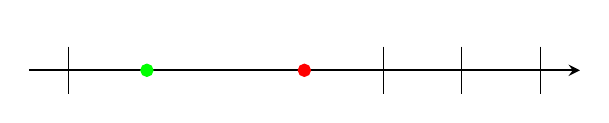
\begin{tikzpicture}[node distance=2cm,thick,every node/.style={transform shape}]
      \draw [thick,->,>=stealth] node [above,black] {} (-1,0) -- (6,0);
      \draw [thin] (-0.5,0.3) node [above,black] {$\xSS$} -- (-0.5,-0.3);
      \draw[mark=*,mark size=2pt,mark options={color=green}] plot coordinates {(0.5,0)};
      \draw[mark=*,mark size=2pt,mark options={color=red}] plot coordinates {(2.5,0)};
      \draw [thin]  (3.5,0.3) node [above,black] {$\xBL$} -- (3.5,-0.3);
      \draw [thin]  (4.5,0.3) node [above,black] {$\xSE$} -- (4.5,-0.3);
      \draw [thin]  (5.5,0.3) node [above,black] {$\xNC$} -- (5.5,-0.3);
    \end{tikzpicture}
    \caption{Dynamic entity has creation and deletion dates before the bulk load cut off. This entity is not serialized.}
    \label{fig:cond-1}
    \end{subfigure}
  %
    \begin{subfigure}{\linewidth}
    \centering
    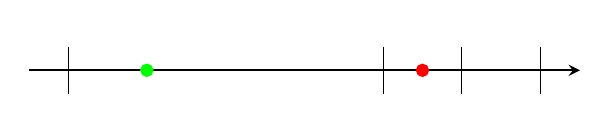
\begin{tikzpicture}[node distance=2cm,thick,every node/.style={transform shape}]
      \draw [thick,->,>=stealth] node [above,black] {} (-1,0) -- (6,0); % timeline
      \draw [thin] (-0.5,0.3) node [above,black] {$\xSS$} -- (-0.5,-0.3);
      \draw[mark=*,mark size=2pt,mark options={color=green}] plot coordinates {(0.5,0)};
      \draw [thin]  (3.5,0.3) node [above,black] {$\xBL$} -- (3.5,-0.3);
      \draw[mark=*,mark size=2pt,mark options={color=red}] plot coordinates {(4,0)};
      \draw [thin]  (4.5,0.3) node [above,black] {$\xSE$} -- (4.5,-0.3);
      \draw [thin]  (5.5,0.3) node [above,black] {$\xNC$} -- (5.5,-0.3);
    \end{tikzpicture}
        \caption{Dynamic entity has creation date before the bulk load cut off and a deletion date after the bulk load cut off, but before the simulation end. Such an entity is serialized into the bulk load component and spawns a delete operation.}
    \label{fig:cond-2}
  \end{subfigure}
  %
    \begin{subfigure}{\linewidth}
    \centering
    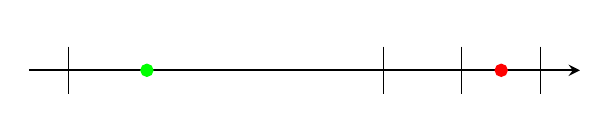
\begin{tikzpicture}[node distance=2cm,thick,every node/.style={transform shape}]
      \draw [thick,->,>=stealth] node [above,black] {} (-1,0) -- (6,0); % timeline
      \draw [thin] (-0.5,0.3) node [above,black] {$\xSS$} -- (-0.5,-0.3);
      \draw[mark=*,mark size=2pt,mark options={color=green}] plot coordinates {(0.5,0)};
      \draw [thin]  (3.5,0.3) node [above,black] {$\xBL$} -- (3.5,-0.3);
      \draw [thin]  (4.5,0.3) node [above,black] {$\xSE$} -- (4.5,-0.3);
      \draw[mark=*,mark size=2pt,mark options={color=red}] plot coordinates {(5,0)};
      \draw [thin]  (5.5,0.3) node [above,black] {$\xNC$} -- (5.5,-0.3);
    \end{tikzpicture}
        \caption{Dynamic entity has creation date before the bulk load cut off and a deletion date after the simulation end. Such an entity is in serialized only into the bulk load component.}
    \label{fig:cond-3}
  \end{subfigure}
    %
    \begin{subfigure}{\linewidth}
    \centering
    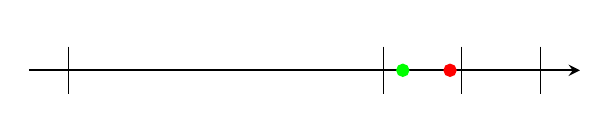
\begin{tikzpicture}[node distance=2cm,thick,every node/.style={transform shape}]
      \draw [thick,->,>=stealth] node [above,black] {} (-1,0) -- (6,0); % timeline
      \draw [thin] (-0.5,0.3) node [above,black] {$\xSS$} -- (-0.5,-0.3);
      \draw [thin]  (3.5,0.3) node [above,black] {$\xBL$} -- (3.5,-0.3);
      \draw[mark=*,mark size=2pt,mark options={color=green}] plot coordinates {(3.75,0)};
      \draw[mark=*,mark size=2pt,mark options={color=red}] plot coordinates {(4.35,0)};
      \draw [thin]  (4.5,0.3) node [above,black] {$\xSE$} -- (4.5,-0.3);
      \draw [thin]  (5.5,0.3) node [above,black] {$\xNC$} -- (5.5,-0.3);
    \end{tikzpicture}
    \caption{Dynamic entity has creation date after the bulk load cut off and a deletion date before the simulation end. Such an entity produces an insert operation and a delete operation.}
    \label{fig:cond-4}
  \end{subfigure}
    %
    \begin{subfigure}{\linewidth}
    \centering
    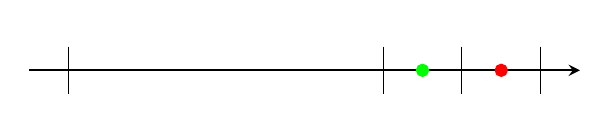
\begin{tikzpicture}[node distance=2cm,thick,every node/.style={transform shape}]
      \draw [thick,->,>=stealth] node [above,black] {} (-1,0) -- (6,0); % timeline
      \draw [thin] (-0.5,0.3) node [above,black] {$\xSS$} -- (-0.5,-0.3);
      \draw [thin]  (3.5,0.3) node [above,black] {$\xBL$} -- (3.5,-0.3);
      \draw[mark=*,mark size=2pt,mark options={color=green}] plot coordinates {(4,0)};
      \draw [thin]  (4.5,0.3) node [above,black] {$\xSE$} -- (4.5,-0.3);
      \draw[mark=*,mark size=2pt,mark options={color=red}] plot coordinates {(5,0)};
      \draw [thin]  (5.5,0.3) node [above,black] {$\xNC$} -- (5.5,-0.3);
    \end{tikzpicture}
        \caption{Dynamic entity has creation date after the bulk load cut off, but before the simulation end, and a deletion date after the simulation end. Such an entity produces only an insert operation.}
    \label{fig:cond-5}
  \end{subfigure}
  \caption{Possible dynamic entity \emph{creation} \textcolor{green}{$\bullet$} and \emph{deletion} \textcolor{red}{$\bullet$} dates with respect to simulation start, bulk load cut off, simulation end, and network collapse.}
  \label{fig:example-graph}
\end{figure}
